\documentclass[conference]{IEEEtran}
\usepackage{graphicx}
\usepackage{times}
\usepackage{subfigure}
\usepackage{url}

\begin{document}

\title{Six ways to understand monads\\
\small{Experiences from the functional programming course at TU Delft}}

\author{\IEEEauthorblockN{Erik Meijer and Georgios Gousios}
\IEEEauthorblockA{
Software Engineering Research Group\\
Delft University of Technology\\
Delft, The Netherlands\\
Email: \{h.j.m.meijer, g.gousios\}@tudelft.nl
}
}
\maketitle

\begin{abstract}

  In the last few years, the popularity of functional programming as a way of
  solving computational problems has increased significantly. While most
  computer science curricula do include a course on functional programming, in
  many cases it is disconnected from practical applications, which is
  precisely where functional programming shines. To fill in this gap, we
  designed a functional programming course that  required students to
  learn by experience with real world applications. In this paper, we present
  the course's design and outline our experience from delivering it.

\end{abstract}

\begin{IEEEkeywords}
functional programming, teaching
\end{IEEEkeywords}

\section{Introduction}

Due to a variety of reasons, including the advent of cloud computing, the rising
rate of information production and the necessity to reach the market fast,
currently, large corporations and start-ups alike are investigating alternative
programming and information storage models. As a result, during the last few
years, the practical software engineering field is witnessing a noticeable shift
towards functional programming. Scripting languages, notably Javascript and
Ruby, pioneered the introduction of functional concepts, such as closures and
lambda functions, to mainstream programming. A new wave of programming
languages, developed to overcome the expressiveness and complexity limitations
exhibited in mainstream languages, have promoted functional constructs, such as
type safe pattern matching, higher order functions and single assignment
variables, to first class citizens (Scala, {\sc c\#}).  New, functional
languages have emerged to fill in the remaining gaps (F\#, Clojure, Racket),
often introducing significant advancements in their field of specialisation
(such as Erlang in distributed fault-tolerant systems).  Finally, large scale
information processing systems such as Map/Reduce~\cite{Dean04} and domain
specific languages such as {\sc linq} have integrated functional concepts to
ease the expression of masively parallel computations.

Broadly speaking, functional programming is a style of programming in which the
primary method of computation is the application of functions to arguments.
Among other features, functional languages offer a compact notation for writing
programs, powerful abstraction methods for structuring them, and a simple
mathematical basis that supports reasoning. Many of the advanced techniques in
modern functional languages, such as monads and catamorphisms, are closely based
on principles from category theory such as functors, initial algebras, monads
and Kleisli categories.

While functional programming has been taught for long in computer science
departments~\cite{Joost93}, curricula tend to emphasize functional programming
theory rather than practical applications. Special programming languages are
used to teach functional programming specific concepts, while little connection
is made to how those concepts can be transfered to non-functional languages.
The course at TU Delft attempted to teach functional programming principles in the
classroom and then expect students to apply those concepts in the (non-purely
functional) language of their choice. The course had a very strong teaching by
example focus: students were expected to participate in both in-classroom
exercises, homework assignments and implement a real world system as a final
project.

\section{Challenges}

While planning the course, we dealt with the following challenges related
to the course's organization and content.

\subsection{Heterogeneous background of participants}

The functional programming course is elective at the MSc level. Students
from all departments in the Electrical Engineering, Mathematics and Computer
science faculty are allowed to participate. For practical reasons, the
enrollment to the course was limited to 15 participants. This permitted
us to get to know the students individually and to provide them with
personalized support.

From the students that enrolled, most have received formal introduction to
imperative and object oriented programming in their bachelors curriculum, while
through participation to other courses they had limited exposure to functional
programming (i.e. Map/Reduce in the web information systems
course). Two of the students were majoring in computer engineering, which meant
that their programming experience was restricted. Several students also had work
experience as programmers as part of their industrial placement or through
participation to start up ventures.

The diverse backgrounds of the students guaranteed that no generic
introduction to the topic would be sufficient. For this reason, we decided
to adopt a hands-on-first approach; the students would have to learn by
flexing their programming muscles, instead of being introduced to 
the theory through toy examples.

\subsection{Choosing the appropriate topics}

Functional programming is arguably one of the oldest programming paradigms. In it is
purest form, it is based on a minimalistic theoretical background
($\lambda$-calculus). Relatively recent
formulations~\cite{Meije91, Wadle93} also introduced concepts from category
theory. While the every day use of functional programming does not necessarily
require the programmer to be aware of the theory, understanding it usually leads
to more elegant algorithmic solutions. Functional programming teaching is also
associated with advanced type systems; indeed, the flagship functional
programming languages (Haskell and the {\sc ml} family) both offer very
sophisticated support for types. Consequently, teaching the full spectrum of
functional programming theory and techniques would have been impossible in a
half-semester course; instead we decided to focus on practical aspects of data
processing, transformations and state representation using functional
techniques.

\subsection{Choosing the appropriate programming language}

Programming languages, in addition to enabling the programmer to express a
series of instructions to be executed by a computer, affect the programmer's
thought process and consequently her approach towards problem
solving~\cite{Ivers80}.  When teaching a programming course, it is important to
be able to demonstrate concepts without interference by the chosen language's
syntax. However, a non-practical language might have the opposite effect; our
experience has shown that the further a demonstration language is from practical
application, the less important students feel the taught concepts are.
Fortunately, most functional programming concepts can be expressed cleanly by
several widespread languages: for example, Javascript, Ruby and {\sc c\#} have
closures, first class and higher order functions, while a number of emerging
languages, such as Scala, Racket, {\sc f\#} and Clojure are functional languages
implemented on familiar development platforms. Apart from staying compatible
with the existing literature, there is no practical reason that necessitates
teaching strictly in a language like Haskell or {\sc ml}.

The above led us to not choose any particular language for the course.  During
the lectures, the demonstration languages where Haskell and {\sc c\#}, while at
the labs we used Scala. We actively encouraged students to use the language of
their choice on the platform of their choice to carry out homework assignments
and the course's final project.

\section{The Course}

The high level goal of the course was to teach the principles of functional
programming, and the corresponding Category theoretical principles. 
More specifically, the educational purposes of the course were:

\begin{itemize}

  \item To introduce students to basic functional programming concepts,
    higher order functions, monads and advanced type systems.

  \item To introduce students to the approach of expressing data processing
    problems as a series of function applications.

  \item To explain the application of functional concepts in non-purely
    functional environments.

\end{itemize}

The course consisted of a series of lectures, of which two where invited
lectures by an external instructor, and laboratory sessions. In total, the
course consisted of 14 hours of lectures and 8 hours of lab work.
The students
also had to carry out a series of homework assignments and a final project.
The evaluation would be based on student performance on the final assignment. 
The lectures took place in a quarter (half semester), during 3 intense 
weeks; the students had another 6 weeks to finish their final projects.

\subsection{Lectures}

The lectures covered the following topics:

\begin{itemize}

  \item Functions and functional composition, higher order functions, recursion, 
    avoiding recursion via higher order functions.

  \item Basic types, function types, currying.

  \item Lists, mapping and traversal using folds.

  \item Monads, composition and their application on the {\sc linq} query 
    language~\cite{Meije11}.

  \item Monoids, functors and their application on data structure processing.

  \item Functional formalization of the Map/Reduce data processing
    paradigm~\cite{Lamme08}.

\end{itemize}

The lecture material was loosely based on Graham Hutton's functional programming
course at the University of Nottingham. The course's recommended book was
Programming in Haskell by the same author~\cite{Hutto07}.

\subsection{Student projects}

At the end of the lecture period, the students were given a selection of
projects to work on. The projects included:

\begin{itemize}

  \item Real time graph visualisation on steaming data. The
    particular example that students worked on was visualizing community
    structures for Github projects.

  \item Multi-source real time data processing. Students worked on a 
    programming language popularity index, based on data from the Github
    event stream and the StackOverflow tag cloud {\sc api}.

  \item Implementation of Haskell constructs in Javascript. Students implemented
    the Haskell Prelude (basic functions for list manipulation).

  \item Implementation of Map/Reduce algorithms in Haskell. Students installed
    and configured cloud Haskell and implemented simple Map/Reduce based
    algorithms in a distributed setting.

  \item Implementation of simple constraint solvers.
  
  \item Machine learning algorithms. Students implemented Na\"ive Bayes 
    classifiers and K-means clustering algorithms.

\end{itemize}

To counterbalance the differences in student experience level, 
the assignments were open ended; students could drive their projects as
far as they where willing to.
The deliverables for the assignments were a repository
with the source code and short report describing the solution that the
students came up with. The students were also required to present a working
demo by the end of the course time. 

\subsection{Labs}

The purpose of the lab sessions where to help students carry out their final
assignments and further explain concepts that might not be clear to students. 
Students convened every week, presented their progress and discussed with 
each other and with the lab demonstrator design and practical issues that
arised in the implementation of their projects. To further motivate students
to work on their projects, one of the lab sessions was converted to a full
day coding sprint.

\section{Experiences}

\subsection{Teaching by example}

The focus of teaching was to present functional programming from a practical
aspect; we were mostly interested to teach students what they can do rather than
the theory behind functional constructs. An important distinction that was made
early on was that the world is imperative; therefore while functional
programming can be a great tool for thinking about a problem, a pure functional
solutions cannot reflect on the real world. As a consequence, it is usually best
to mix programming paradigms, i.e. imperative or object-oriented programming for
state representation and functional programming for data processing. In our
experience, this distinction helped students understand that they are already
doing functional programming without noticing; enforcing data immutability to
handle multi-threading problems or passing function arguments in scripting
languages are applications of functional programming principles. The moment
students realized this fact, their attention was captured to the lectures.

During both lectures and labs, all non-whiteboard examples where actually
entered in a real programming environment (LinqPad or the Scala command line
read-evaluate loop) and the results of the evaluation where discussed with the
students. Participation was encouraged by modifying the examples and asking the
students to perform the evaluation, before the example was executed. The
examples varied from list manipulation with higher-order functions to 
a toy actor model example.

The proverbial ``six ways to understand monads'' included presentations of the
formal theoretical concepts, visualizations of monads as blenders (based on the
monadic property that once a value is captured, it is then contained),
applications in Haskell for encapsulating state (through the \textsf{Maybe}
monad), applications to generic programming in {\sc c\#}, applications to {\sc
linq} and the reactive extensions frameworks, and, finally, a whiteboard
exercise where students were prompted to participate in the ad-hoc specification
of Haskell's \textsf{IO} monad from basic principles. Once again, the examples
enabled the students to understand the composition and state containment
properties of an otherwise difficult to comprehend theoretical concept.

\subsection{The teapot exercise}

\begin{figure*}
\centering
\label{fig:teapots}
\subfigure[Input drawing, rendered with Java graphics]{
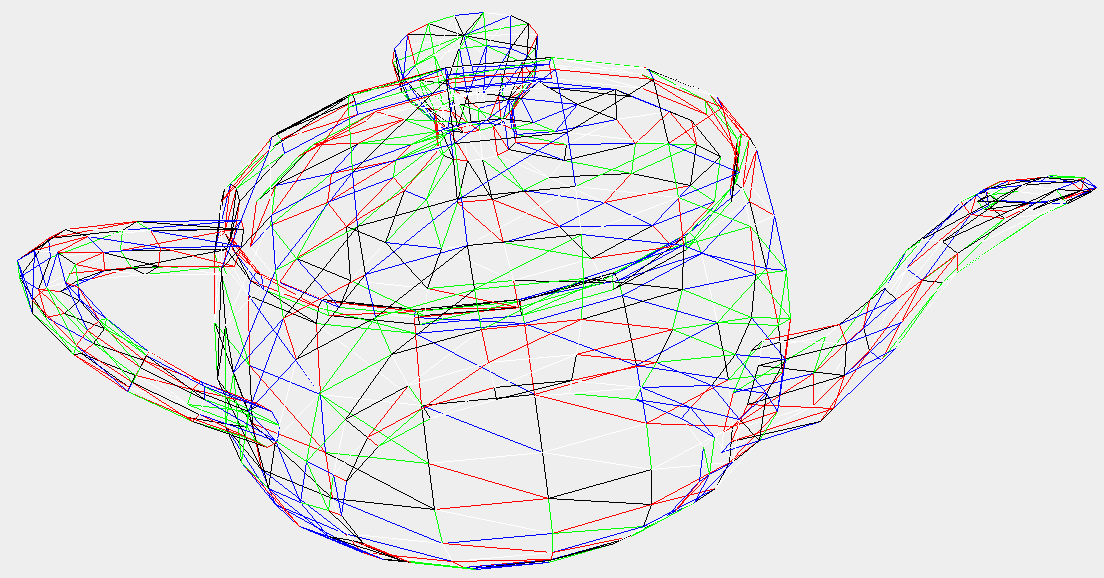
\includegraphics[scale=0.173]{teapot-reference.png}
\label{fig:teapot-reference}
}
\subfigure[Decomposition in Scala, rendered with Java graphics]{
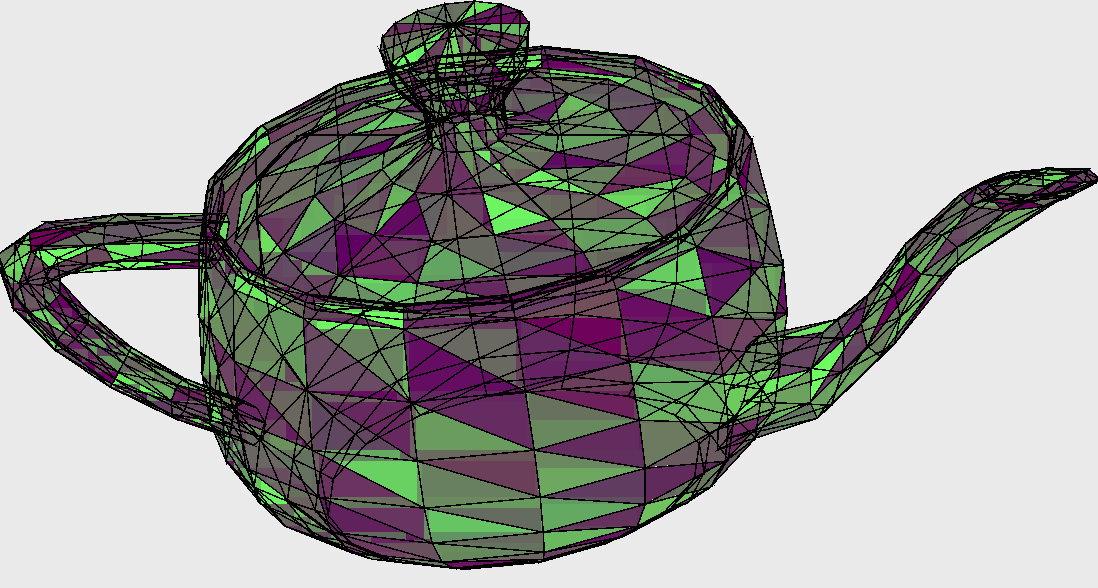
\includegraphics[scale=0.17]{teapot-java-canvas.png}
\label{fig:teapot-scala}
}
\subfigure[Decomposition in Scheme, rendered with appropriately positioned {\sc html} \textsf{div}
elements]{
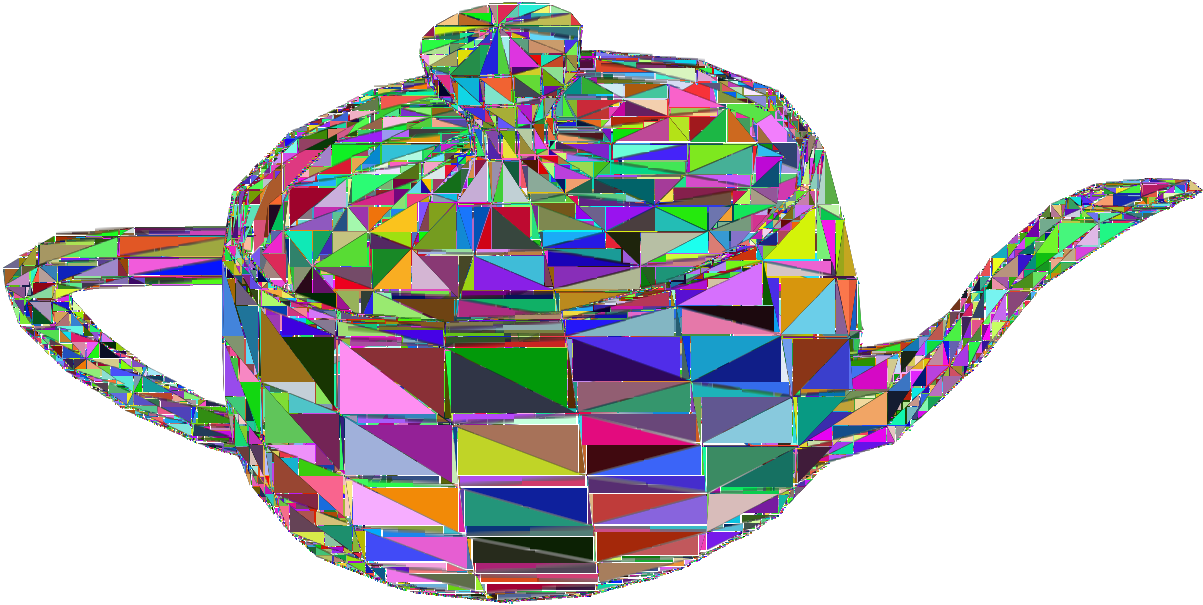
\includegraphics[scale=0.195]{teapot-html-divs.png}
\label{fig:teapot-html-divs}
}
\subfigure[Decomposition in Javascript, rendered with {\sc html5} graphics]{
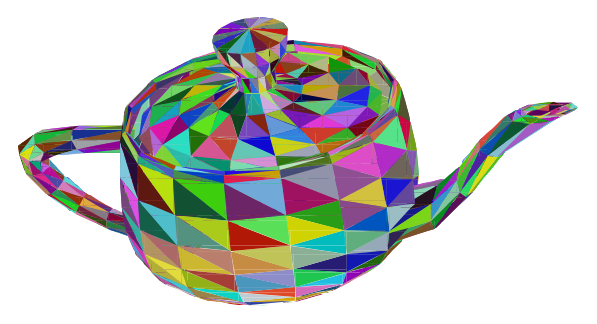
\includegraphics[scale=0.295]{teapot-html-canvas.png}
\label{fig:teapot-html-canvas}
}
\caption[]{Example results from the teapot exercise.}

\vspace{-1.5em}
\end{figure*}

One of the highlights of the taught period of the course was the teapot
exercise, which we used it to draw the student's attention to the following
facts:

\begin{itemize}

  \item Most modern programming languages can express functional programming
    constructs.

  \item Functional programming works best in data transformation scenarios.

  \item Complex problems can be solved by decomposing them into smaller and simpler ones.

\end{itemize}

The exercise consisted of rendering the Utah Teapot~\cite{Torre06} using any
graphics primitive of the student's choice using only right triangles (with one
horizontal leg).  In its
core, the exercise required students to decompose a collection of arbitrary triangles, which
comprised the input Utah Teapot model, to a collection of right triangles. The students
had to come up with the decomposition method (using some simple analytic
geometry, this was not a course on 3D graphics), a decomposition termination criterion to stop the decomposition when
triangles were too small to be rendered on screen and a method to recursively
apply the above mentioned transformations on the input data. As always, the
students could decide the implementation language of their choice. The exercise
was given as a mid-week homework assignment, between the Monday and the Friday
lectures.

The student's response was overwhelming. Even though it was made clear that the
exercise would not contribute to the final grade, the will to apply the data
processing techniques taught during the lectures motivated the students to work
very hard. The fact that they were instructed to use their favourite language
enabled them to focus on decomposing the problem in a series of testable
calculation steps rather than meddling with the intricacies of learning a new 
language. In spite of the advice, students were eager to test-drive the newly
acquired knowledge using a functional language; apart from {\sc c\#} and
Javascript, solutions were also provided in Scala, Scheme and Haskell. Example
renderings produced by student programs can be seen in Figure~\ref{fig:teapots}.

\subsection{Map/Reduce}

According to many students, the Map/Reduce data analysis framework was what
drove them to attend the course. The lecture on Map/Reduce featured an invited
talk by Prof. Ralf L\"ammel, who presented his formulation of Map/Reduce using
functional programming principles~\cite{Lamme08} and explained how those can be
applied to process semi-structured data. The talk resonated to students; in
their projects, students used implicit, through the selected language's library
collection methods, or explicit, by formalizing data processing as a series of
in memory Map/Reduce operations, forms of Map/Reduce to process their datasets.
Out of personal interest, one student even implemented L\"ammel's Map/Reduce
formulation in Scala, and through the language's extension mechanisms, adapted
it for use as an extension method by any Scala collection type, including
parallel collections. 

\subsection{The coding sprint day}

Coding sprints or ``hackathons'' have long been used by open source software
projects to speed up development and increase participation of community
members. In a typical sprint, project members set measurable
targets and work intensively in a tight deadline to deliver them. To ensure the
timely delivery of the student projects, we organized an one day coding sprint,
during which the students were requested to i) set explicit targets ii) write
code for 7 hours with a short break iii) present a 5 minute demo of their work
at the end of the day. All project teams where expected to work in the same
room, while communication among the teams was facilitated by the lab
demonstrator, to avoid unnecessary distractions.

Interestingly, the coding sprint was organized on student request. The reason
was that pressure from other courses did not allow them to be together as teams.
The sprint taught students the importance of setting realistic development goals
and the necessity of iterative development. Even though all teams were off
target at the end of the day, most were able to create a rough prototype in less
than 7 hours, using functional programming techniques. 

%\subsection{The student projects}
%
%For implementing their projects, the students selected languages and frameworks
%that are currently emerging and popular among non-traditional software
%development environments. All students did their projects in either Scala or
%Javascript, with one exception, using frameworks such as Akka (for actors),
%Scalatra (for implementing {\sc rest} {\sc api}s) or Node.js (for server-side
%processing). From the implementations it appears that students did apply
%their 
%
\section{Conclusion}

Teaching the concepts of solving problems algorithmically can be a daunting
task~\cite{Futsc06}; especially more so, when the subjects are already in a
specific mindset. The assumption of the presented course was that imperative and
functional programming are really the two sides of the same coin; by focusing on
how students can apply rather than just be taught concepts of functional
programming using the, typically imperative, languages they already know, allows
them to better appreciate the strong points and weaknesses of each paradigm. In
our experience, the approach has been successful. Both throughout the initial
homework assignments and in their projects, the students demonstrated a high
degree of appreciation of functional programming concepts. Above all, we
believe that it was the hands-on approach 
employed in this course that allowed students to sharpen their skills and
understand the concepts that were taught during it.

\section*{Acknowledgements and Availability}
We would like to thank the course participants for their enthusiasm and
dedication. The source code to all student projects and the teapot
exercise can be found at (or linked from) \url{http://swerl.tudelft.nl/bin/view/Main/FunctionalProgrammingCourse}. This work is partially supported by
Marie Curie {\sc ief} 298930 -- {\sc sefunc}.

\bibliography{paper}
\bibliographystyle{ieeetr}
\end{document}

